\documentclass[tikz, 12pt]{article}

\usepackage[margin=1.5in]{geometry}
\usepackage[table]{xcolor}
\PassOptionsToPackage{hyphens}{url}\usepackage{hyperref}
\usepackage{tikz}
\usepackage{graphicx}
\usepackage{amsmath}
\usepackage{caption}
\usepackage{amssymb}
\captionsetup{justification=raggedright,singlelinecheck=false,format=hang}
\usepackage[T2A]{fontenc}
\usepackage[utf8]{inputenc} 
\usepackage{blindtext}
\usepackage{authblk}
\usepackage{listings}
\usepackage{blindtext}
\usepackage{amsthm}
\usepackage{algorithm}
\usepackage{algpseudocode}
\usepackage{lipsum}
\newcommand*\samethanks[1][\value{footnote}]{\footnotemark[#1]}
\renewcommand{\labelenumii}{\theenumii}
\renewcommand{\theenumii}{\theenumi.\arabic{enumii}.}
\usetikzlibrary{positioning,fit,calc,arrows}
\tikzset{block/.style={draw,thick,text width=2cm,minimum height=1cm,align=center},
         line/.style={-latex}
}
\theoremstyle{definition}
\newtheorem{defn}{Definition}
\theoremstyle{remark}
\newtheorem*{remark}{Remark}
\title {Gamechannel}
\author {Alisa Chernyaeva\thanks{Maria}}
\author{Ilya Shirobokov\samethanks} 
\author{  Alexander Davydov\samethanks}
%\author[add1]{Ilia Shirobokov}
\affil{Research department, DAO.Casino Company}
\affil{ \href{mailto:Research@Dao.casino}{Research@Dao.casino}}
%\address[add1]{Research department, company DaoCasino}
\date {August 2018}
\hyphenation{every-where}
\begin{document}
\maketitle
	\begin{abstract}
State Channel is a technology designed for scaling blockchain projects; it allows reduces the number of transactions and accelerates the transaction exchange. On the basis of this technology DAO.Casino developed its own Game Channels tailored to the needs of the gambling segment. This ad hoc solution embraces functionality for generating provably fair numbers and for delegating blockchain interaction to a third party. This article covers: the set protocols behind Game Channel implementation, the random number generation algorithm based on the digital signature scheme, and modifications for the original concept. Note that the application area of the Game Channel technology is not supposed to be limited to the gambling segment and can be implemented for diverse game types.

	\end{abstract}
\tableofcontents	
	\input{sections/Introduction}
	\section{Preliminaries}
In this section we introduce definitions and notation that will be used throughout the paper.

We denote the set of integers modulo an integer $n$ by $\mathbb{Z}_n$. When writing $x \xleftarrow{\text{R}} S$ we mean that $x$ is chosen uniformly at random from the set $S$. By $H$ we denote some cryptographic hash function. 

The communication model considers a point--to--point channel between two parties. One of them may be a malicious adversary. The adversary can diverge from the specified protocol in any way. 

	\subsection{Safety and liveness of game channels}

Liveness of game channels assures that there is always a result for each of the channel participants within a round. Round results within the channel can be saved on--chain any time,  with a submission window of sufficient size left to avoid miner attacks. Thus, game channels rely on the blockchain liveness. Simply put, the exact state sent by the channel participants must always be locked in the blockchain. It is assumed that the state is accepted and signed by all channel participants. Given the above, it is important that all participants have stable Internet connections free of significant interruptions. 

The safety of a game channel also relies on the safety of the blockchain. It assures that all game channel participants obtain a valid and identical result. Analyzing intra--channel activities, we can suggest a case when a participant does not respond to messages sent to him via the channel. There is no telling whether an actual network failure occurred or a participant deliberately gave no response. As far as state channels are concerned, the participant availability issue is expected to be resolved through implementing some procedure for obtaining a valid result even when one of the participants is unavailable. In game channels the relevant functions are integrated into the smart contract responsible for dispute resolution; the smart contract is authorized to decide the reward distribution in compliance with the game logic. Note that a new round can only be started after all the parties have agreed upon the previous round. Thus, in the worst case one player will be in the $n+1$ state, while the other is in the $n$ state. If the first player fails to send a state update, the dispute is resolved in favor of the second player, who receives the maximum reward.

\textit {Griefing} is the ability of a participant to deviate from the protocol in order to disrupt participant interaction without directly violating the security of the protocol. There are two griefing strategies. One implies forcing a party into paying the channel closure transaction; to do so, a party that was supposed to close the channel does not send the transaction to the blockchain. This is not a major issue, as state deposits considerably exceed transaction costs, and participants are likely to assume this risk. The other strategy implies posting expired channel states during a dispute if an attacking party believes that the other participant is unavailable. To reduce this risk, a game channel checks the game round number when there is a state change attempt in dispute; if the difference between the round number of the new state and the round number suggested by an attacker exceeds 1, the attacker loses their deposit.

It is noteworthy that an incorrect implementation of game channels and software errors can cause one or both players to lose their entire deposits. However, this issue is out of the scope of the present work.

	\subsection{Signatures and Fingerprints}
\begin{defn}
A signature scheme $ \Sigma $ is a tuple $(M, S, K, KeyGen, Sign, Verify)$ where:
	\begin{itemize}
		\item $ M $ is a finite field of possible messages;
		\item $ S $ is a finite field of possible signatures;
		\item $ K $ is a finite field of possible keys;
		\item $ KeyGen: (1^k) \rightarrow (sk, pk) $. This algorithm takes as input a security parameter $k$ and outputs secret and public keys;
		\item $Sign_{sk}: (m) \rightarrow \sigma $. The signing algorithm takes as input a message $m \in M$ and secret key $sk \in K$, and outputs a signature $\sigma \in S$;
	\item $Verify_{pk}: (m, \sigma) \rightarrow \{0, 1\} $. This algorithm check whether the signature $\sigma \in S$ for a message $m \in M$ and a public key $pk \in K$ is valid.
	\end{itemize}
\end{defn}
In addition we define the uniqueness property for a signature scheme. 
\begin{defn}
A signature scheme $ \Sigma $ is called \textit{unique} if for every message $m \in M$ and for every public key $pk \in K$ there is only one valid signature $\sigma \in S$.
\end{defn}

In our protocols we use two types of signature schemes: RSA \cite{bib19} and ECDSA \cite{bib20}. ECDSA is a standard signature for transaction acknowledgement within a channel. RSA is reserved for pseudorandom number generation in the Signidice algorithm.

\begin{remark}
RSA can be replaced by any other signature with the uniqueness property. We suggest considering BLS \cite{bib10} as the primary alternative.
\end{remark}

When a channel is open, the smart contract only stores the \textit {Merkle--tree fingerprint} and not the entire RSA public key. The purpose of this is to reduce the transaction cost of opening a channel.

\begin{defn}
Let $pk = (N, e)$ be a RSA public key. Then $f = H(H(e), H(N))$ is a Merkle--tree fingerprint of the RSA public key $pk$. 
\end{defn}
\begin{remark}
In the DAO.Casino implementation $KECCAK-256$ \cite{bib21} is always used for the $H$ function to ensure compatibility with Ethereum. 
\end{remark}

	\subsection{Signidice}

Signidice \cite{bib18} is a protocol that allows pseudorandom number generation by two parties. 

Define the bit hash length as $hash.size$, and the maximum and the minimum number the generation can yield as $max$ and $min$ respectively.

\begin{algorithm} 
%\floatname{algorithm}{Signidice} %
\caption*{$\textbf{Signidice}$} \label{alg:signidice}
\begin{algorithmic}
\State 1. $ Alice \ \text{send}\  seed\xleftarrow{\text{R}} \{0,1\}^* \  \ \text{to} \ Bob$
\State 2. Bob computes:
\State $\ \ \ \ h \gets H(seed)$
\State $\ \ \ \ S \gets  \Sigma . Sign_d(h)$
\State $\ \ \ \ L \gets H(S) $
\State $\ \ \ \ range \gets max - min +1$
\While {$L \geq \left\lfloor (2^{hash.size}-1) / range\right\rfloor \cdot range $}
\State$ L \gets H(L)$
\EndWhile
\State $ \ \ \ \  L \gets (L \bmod range) + min $
\State 3. $Bob \ \text{send}\  S, \ L \ \   \text{to} \ Alice$
\State 4. Alice check results:
\If {$ \Sigma .Verify_e(S) \ \text{and} \  L \ \text{is correct}$}  
\State The number L is accepted
\Else 
\State The number L is not accepted
\EndIf
\end{algorithmic}
\end{algorithm}

\begin{remark}
If  $max -  min$ is a power of two, the while loop in step 2 of the Signidice algorithm can be omitted. But if it isn't a power of two, the resulting distribution is not uniform, as some numbers may be more likely than others.
\end{remark}

In the DAO.Casino implementation the unique RSA unique signature is used by the $Sign$ and $Verify$ functions:
\begin{itemize}
	\item $RSA.Sign_d(m): \mathbb{Z}_n \rightarrow \mathbb{Z}_n: m \rightarrow m^d mod N$
	\item $RSA.Verify_e(m, s): \mathbb{Z}_n \times \mathbb{Z}_n \rightarrow \{True, False\}: (m, s) \rightarrow \text{check if } \\ s^e mod N == m $
\end{itemize}

	\subsection{Channels}
As stated above, State Channel operation requires an on--chain smart contract. Let’s define the core functionalities required to enable this contract:
\begin{itemize}
	\item $ OpenChannel $ - Defines the parties’ consent to interact within the channel;
	\item $ UpdateChannel $ - Changes the last state stored in blockchain to the newest state approved by both parties;
	\item $ CloseChannel $ - Completes the channel operation. The latest state approved by both channel parties is stored in the blockchain; funds are distributed according to the state;
	\item $ OpenDispute $ - The game is halted and a dispute is initiated when one of participants fails to get reliable relevant data. A dispute has two potential outcomes specified below;
	\item $ ConsensusResolve $ - Parties resolve the dispute by consenting a new state;
	\item $ ArbitrationResolve $ - The dispute is resolved through smart contract arbitrage.
\end{itemize}

\begin{remark}
Note that these functionalities may be implemented within a single contract or within several interacting contracts.
\end{remark}

Now we introduce the following concept. 
\begin{defn}
The set $ (OpenChannel, UpdateChannel, CloseChannel,\\ OpenDispute,  ConsensusResolve, ArbitrationResolve) $
is called a \textit {Game Channel Contract System} and is denoted by \textit {GCCS}. 
\end{defn}

\begin{remark}
GCCS can also be extended by adding additional functionality, but these addons are out of scope in the present work. 
\end{remark}

\begin{defn}
We say that a connection between two parties is called a \textit {Сhannel} if the following conditions holds:
	\begin{enumerate}
		\item Every message sent contains some game--related data;
		\item Every message (or main part of a message) is signed by the sender;
		\item The connection verified by GCCS. 
	\end{enumerate}
\end{defn}

Each channel has a $state$. The channel state is the last message sent by a participant that unambiguously defines the latest game state and/or the participants' balance. Note that each protocol participant must store the latest channel state. 

Also, each channel has a $lifetime$ parameter. The $Lifetime$ defines the number of blockchain blocks available to the GCCS to update the channel state and open disputes related to this state. 

We define the channel participants as: $Player$ and $Dealer$. The table below defines the differences between these roles:
\begin{center}
\begin{tabular}{ |c|c| } 
 \hline
 \textbf{Player} & \textbf{Dealer} \\ 
 \hline
 Makes bets & Receives bets \\ 
 Generates PRNG seed & Generates pseudorandom numbers \\ 
 Checks game results & Calculates game results\\
 \hline
\end{tabular}
\end{center}
Other differences depend on the specific protocol implementation.

To coordinate different actions within the channel, GCCS must be able to recognize approvals from both parties. If a channel state signed by Player and by Dealer is received, GCCS considers that the participants have reached a consensus. Note that the sender does not matter in this case. To reduce transaction costs, receiving one signature may suffice if the transaction itself is sent by the other party (i.e. approval is confirmed by sending).  

\textit {Channel Status} is a global variable defining the current channel status. The following status values are defined:
\begin{itemize}
	\item $Unused$ - channel wasn't opened before;
	\item $Open$ - channel open, game in progress;
	\item $Close$ - channel was previously used and is now closed;
	\item $Dispute$ - channel is open, dispute in progress.
\end{itemize}

The chart below illustrates the channel life--cycle from state to state.
\\
\\
\begin{center}
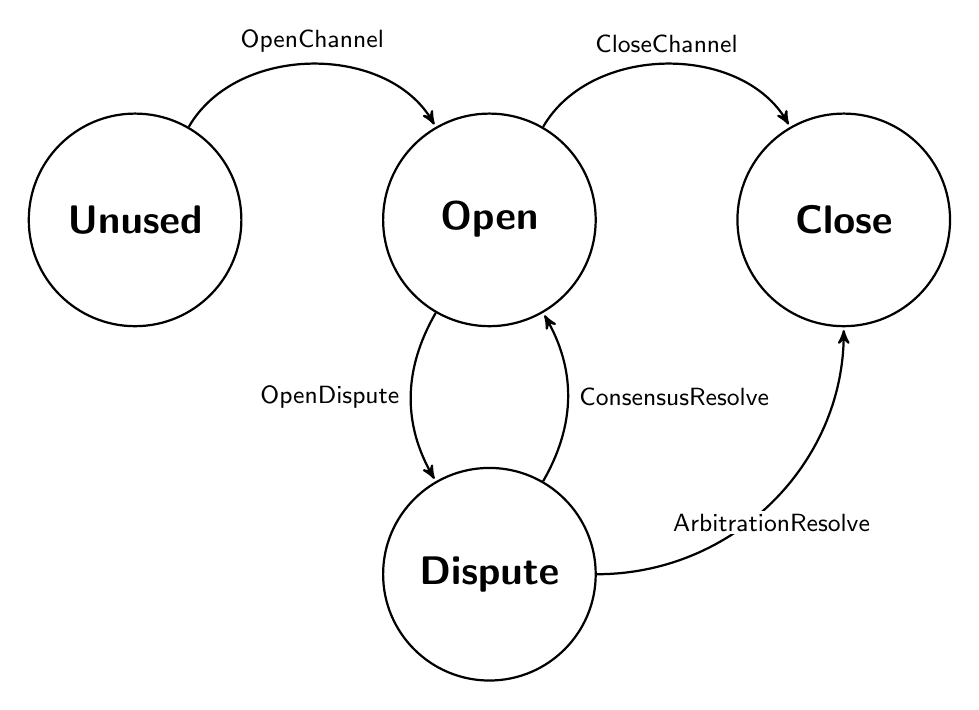
\begin{tikzpicture}[->,>=stealth',shorten >=1pt,auto,node distance=45mm,
  thick,main node/.style={circle,fill=white!20,draw,
  font=\sffamily\Large\bfseries,minimum size=27mm}]

  \node[main node] (unused) {Unused};
  \node[main node] (open) [right of=unused] {Open};
  \node[main node] (close) [right of=open] {Close};
  \node[main node] (dispute) [below of=open] {Dispute};


  \path[every node/.style={font=\sffamily\small,
      fill=white,inner sep=1pt}]
    (unused) edge [bend left=60] node[above=1mm] {OpenChannel} (open)
    (open) edge [bend left=60] node[above=1mm] {CloseChannel} (close)
    (open) edge [bend right=30] node[left=1mm] {OpenDispute} (dispute)
    (dispute) edge [bend right=30] node[right=1mm] {ConsensusResolve} (open)
    (dispute) edge [bend right=45] node[below=1mm] {ArbitrationResolve} (close);
\end{tikzpicture}
\end{center}

The dispute state is the same regardless of the underlying cause. After recording this state, the channel can either go back to open or closed depending on parties' actions. The channel goes back to open if parties are able to agree upon a new state. If the dispute is resolved through smart--contract arbitrage, the channel moves to the closed state.

Now we can say that a $ Game \ Channel $ is a channel $\gamma$ such that Player and Dealer use the protocols described in this paper. 


		\section{Game Channels} \label{gamechannel}
In this section we are going to give a detailed coverage of protocols that allow two parties to open a game channel, play a game, close the channel and get rewards facing no risk of counterparty fraud. Also, we are going to consider the dispute resolution mechanism.

By $dk$ and $pk$ denote, respectively, Dealer's and Player's ECDSA keys. 

\begin{table}[h]

\caption{The names of variables and their meanings \\ (Solidity implementation)}
% \rowcolors{1}{lightgray}{white}
\begin{tabular}{|l|c|l|}
\hline
Name&Type&Descriprion\\
\hline
channelId & bytes32 & Unique channel identifier\\ 

playerAddress & address & Player's ethereum-address\\            
dealerAddress & address & Dealer's ethereum-address\\  
gameContractAddress & address & Ethereum-address of the game\\             
playerBalance & uint256 & Player's deposit value\\                   
dealerBalance & uint256 & Dealer's deposit value\\                   
openingBlock & uint256 &  Information identifying when a message sent\\                  
RSAfingerprint & bytes32 &  Merkle-tree fingerprint of the RSA public key\\  
gameData & bytes & Game process data\\
round & uint256 & Round number of the game session \\
bet & uint256 & Player's bet \\
seed & bytes32 & Random seed for PRNG\\
totalBet & uint256 & Total amount of  player bets \\
flag & bool &Closing flag \\
maxNumber, minNumber & uint256 & Boundaries of random numbers in the game\\
\hline
\end{tabular}
\end{table}

\subsection {Opening a channel}
Player initiates the channel open event. To open a channel, its participants have to agree upon a specific initial state and confirm it with their signatures. Then the transaction with a state and participant signatures is sent to the smart-contract that verifies data validity. The smart-contract calculates a unique channel ID generated according to the following formula:
\begin{center}
 $channelId = H(gameContractAddress, playerAddress, dealerAddress, $ \\ $playerBalance, dealerBalance, openingBlock, RSAfingerprint)$.
\end{center}
 Note that either participant may send the opening transaction. For simplicity, let’s assume that it is sent by Dealer. The message exchange sequence is specified in the  \autoref {alg:openchannel} protocol.

\begin{algorithm}
\floatname{algorithm}{Protocol}
\caption{Opening a channel} \label{alg:openchannel}
\begin{enumerate}
	\item Player sends message containing amount of tokens for Player's deposit to Dealer.
\begin{center}
	 $initial\_message\ = (playerAddress, playerBalance, dealerAddress,$\\$ gameContractAddress)$
\end{center}
	\item Dealer generates the public RSA key $RSA\_public\_key= (N,e)$ and calculates the $RSAfingerprint$. Then, Dealer generates the following messages:
\begin{center}
	 $open\_message = (playerAddress,  dealerAddress, playerBalance, $\\$dealerBalance, openingBlock, gameData, RSAfingerprint, gameContractAddress)$

	$dealer\_signed\_message = ECDSA.Sign_{dk}(open\_message)$
\end{center}
	\item Dealer sends the following data to Player:
\begin{center}
$(RSA\_public\_key, open\_message,dealer\_signed\_message)$
\end{center}
	\item Player receives the message, checks data in it and then signs the $open\_message$ and sends it back to Dealer.
\begin{center}
	$player\_signed\_message = ECDSA.Sign_{pk}(open\_message)$
\end{center}
\item If the $player\_signed\_message$ is valid, Dealer calls the $openChannel$ smart contract function with the following data:
\begin{center}
$(open\_message,dealer\_signed\_message,player\_signed\_message)$
\end{center}	
\begin{lstlisting}
    function openChannel(
        playerAddress,
        dealerAddress,
        playerBalance,
        dealerBalance,
        openingBlock,
\end{lstlisting}
\end{enumerate}
\end{algorithm}
\begin{algorithm}
\begin{lstlisting}
	     gameData,
	     RSAfingerprint,
	     gameContractAddress,
	     dealer_signed_message,
	     player_signed_message
 	   )
\end{lstlisting}
\begin{enumerate}
\setcounter{enumi}{5}
\item The contract verifies validity of the received data. If valid, it is assumed that the both parties approved channel opening. Then the contract generates $channelId$ and freezes funds of the both parties for the game. The channel status changes to $Open$. 
\end{enumerate}
\end{algorithm}

\theoremstyle{definition}
\newtheorem{exmp}{Example}[section]
\begin{exmp}
Let’s assume that Bob runs a casino. Alice wants to use Bob’s service to play roulette available in the list of games. First Alice allows the game contract to transfer 100 of Alice's tokens to later use them as a deposit. Then she sends the following message to Bob:
\\
\\
\begin{tabular}{ccc}
   	\begin{tabular}{c}
   	Alice:\\
	$0xde8456...$\\
   	\end{tabular} &
   \begin{tabular}{l}
   $\underrightarrow{ \quad  (0xde8456..., 100,
 0x87ff5a...,\  \quad \quad \quad$ \\  $  \quad 0x8a4654...) \quad}$
   \end{tabular}&
  	 \begin{tabular}{c}
 	 Bob:\\
	$0x87ff5a...$\\
   	\end{tabular} \\
\end{tabular}\\

Bob analyzes the message and agrees to carry out a game. Bob allows the game contract to transfer 5000 of Bob's tokens to later use them as a deposit. Then he responds to Alice:
\\
\\
\begin{tabular}{ccc}
   	\begin{tabular}{c}
   	Alice:\\
	$0xde8456...$\\
   	\end{tabular} &
   \begin{tabular}{c}
   $\underleftarrow{\quad (N, e, 0xde8456..., 0x87ff5a..., 100, \ \quad $ \\  $ \quad 5000, openingBlock, gameData,\quad $ \\  $ \quad  RSAfingerprint, 0x8a4654...,\quad $ \\  $ \quad Bob\_signature ) \quad}$
   \end{tabular}&
  	 \begin{tabular}{cl}
 	 Bob:\\
	$0x87ff5a...$\\
   	\end{tabular} \\
\end{tabular}\\
\\

Alice checks the Bob’s message and, making sure it is valid, signs it on her part and sends back.
\\\
\\
\begin{tabular}{ccc}
   	\begin{tabular}{c}
   	Alice:\\
	$0xde8456...$\\
   	\end{tabular} &
   \begin{tabular}{c}
   $\underrightarrow{\quad (0xde8456..., 0x87ff5a..., 100, 5000, \quad $ \\  $ \quad openingBlock, gameData, \quad $ \\  $ \quad RSAfingerprint,0x8a4654...,\quad $ \\  $ \quad Alice\_signature ) \quad}$ 
   \end{tabular}&
  	 \begin{tabular}{cl}
 	 Bob:\\
	$0x87ff5a...$\\
   	\end{tabular} \\
\end{tabular}\\
\\

Checking Alice’s signature for validity, Bob sends both their signatures to the contract alongside the data about the channel.\\
\begin{tabular}{ccc}
   	\begin{tabular}{c}
 	 Bob:\\
	$0x87ff5a...$\\
   	\end{tabular} &
   \begin{tabular}{c}
   $\underrightarrow{\quad (0xde8456..., 0x87ff5a..., 100, 5000, \quad $ \\  $ \quad  openingBlock, gameData, \quad $ \\  $ \quad RSAfingerprint,0x8a4654...,\quad $ \\  $ \quad Bob\_signature,  Alice\_signature ) \quad}$
   \end{tabular}&
  	 \begin{tabular}{cl}
 	 Contract:\\
	$0x8a4654...$\\
   	\end{tabular} \\
\end{tabular}\\
\\

The smart contract checks validity of the both signatures and the balances of the participants. Then the contract locks the participant deposits. From this moment the channel is open.
\end{exmp}

\subsection {Interaction within the channel}

Once the channel is open, the whole gambling process is divided into rounds. In each round a player takes specific game-related decisions (e.g. makes a bet) and sends them to the dealer with a random seed. On the basis of this seed, the dealer then computes the game result. If the player accepts the obtained result as fair, the next round begins. The process of party interaction with a single round is defined by the \autoref{alg:intchannel} protocol. 

\begin{algorithm}
\floatname{algorithm}{Protocol}
\caption{Messaging in the channel} \label{alg:intchannel}
\begin{enumerate}
	\item Player generates the $seed$ and the following  messages:
\begin{center}
$ seed\_message = (channelId, bet, round, gameData, seed)$
$signed\_seed\_message = ECDSA.Sign_{pk}(seed\_message)$ 
\end{center}
 then sends data to Dealer. 
	\item Dealer checks the $signed\_seed\_message$, $seed\_message$ and computes:
 \begin{algorithmic}
\State $V = H(seed\_message)$
\State $S = RSA.Sign(V)$
\State $S_{hash} = H(S)$
\State $gameRange = maxNumber -  minNumber + 1$
\While {$S_{hash} \geq \left\lfloor (2^{hash.size}-1) / gameRange \right\rfloor \cdot gameRange$}
\State$ S_{hash}\gets H(S_{hash})$
\EndWhile
\State $L = (S_{hash}$ mod $gameRange) + minNumber$
 \end{algorithmic}
 Applying the game logic to the resulting number, Dealer obtains the round result.
\item Dealer signs the new channel state
\begin{center}
$update\_channel\_message = (channelId, playerBalance, dealerBalance, gameData, round)$
$dealer\_signed\_message = ECDSA.Sign_{dk}(update\_channel\_message)$
\end{center}
\item Then Dealer sends the following message to Player:
\begin{center}
 $message = (L,S, update\_channel\_message, $ \\ $dealer\_signed\_message)$
\end{center}
	\item Player makes sure that the number L, the game result and new participants' balances are calculated correctly.
\end{enumerate}
\end{algorithm}


\begin{algorithm}
\begin{enumerate}
\setcounter{enumi}{5}
\item Player sends the $update\_channel\_message$ and its signature back to Dealer. 
\begin{center}
 $player\_signed\_message = ECDSA.Sign_{pk}(update\_channel\_message)$
\end{center}
 \item If the player or the dealer want to update the on-chain state of the game, they call the update channel function of the smart-contract:
\begin{lstlisting}
    function updateChannel(
	channelId ,
	playerBalance,
	dealerBalance,
	gameData,
	round,
	dealer_signed_message,
	player_signed_message
    )
\end{lstlisting}
\end{enumerate}
\end{algorithm}

Note that, every time a channel state is updated, game-related-data is also recorded to the blockchain. It allows us to maintain necessary game-related statistics and to distribute rewards between the casino and the game developer according to actual bets.

\begin{exmp}
Getting back to the above example, Alice places her bet of 10 tokens on red, generates the relevant message and signs it: 
\\
\\
\begin{tabular}{ccc}
   	\begin{tabular}{c}
   	Alice:\\
	$0xde8456...$\\
   	\end{tabular} &
   \begin{tabular}{c}
   $\underrightarrow{\quad (channelId, 10, 1, gameData,\quad \quad \quad \ \ $ \\  $ \quad qw2ert5t, Alice\_signature ) \quad}$
   \end{tabular}&
  	 \begin{tabular}{cl}
 	 Bob:\\
	$0x87ff5a...$\\
   	\end{tabular} \\
\end{tabular}\\
\\

Upon the receipt of the Alice’s message, Bob starts computing the round result. To do it, he calculates hash from Alice’s data and signs it via RSA signature. The result is $0x5r43c...$ Then, on the basis of the obtained number, Bob generates a random number that determines the game result. Let’s assume this number is 14. It is on the red. So, Alice wins the round. Bob generates a message for Alice and signs it:
$update\_channel\_message = (channelId, playerBalance, dealerBalance, gameData, round)$
\\
\\
\begin{tabular}{ccc}
   	\begin{tabular}{c}
   	Alice:\\
	$0xde8456...$\\
   	\end{tabular} &
   \begin{tabular}{c}
   $\underleftarrow{\quad (14, 0x5f43c..., channelId, 110, \quad \quad \quad $ \\  $ \quad 4990, gameData, 1, Bob\_signature) \quad}$
   \end{tabular}&
  	 \begin{tabular}{cl}
 	 Bob:\\
	$0x87ff5a...$\\
   	\end{tabular} \\
\end{tabular}\\
\\

Alice approves the received data upon checking it. She signs the message and sends it to Bob.
\\
\\
\begin{tabular}{ccc}
   	\begin{tabular}{c}
   	Alice:\\
	$0xde8456...$\\
   	\end{tabular} &
   \begin{tabular}{c}
   $\underrightarrow{\quad (channelId, 110, 4990, gameData, 1, \quad $ \\  $ \quad Alice\_signature  ) \quad}$
   \end{tabular}&
  	 \begin{tabular}{cl}
 	 Bob:\\
	$0x87ff5a...$\\
   	\end{tabular} \\
\end{tabular}\\
\\

At the request of either party, the message and both signatures can be sent to the contract to update data stored in it.

Then Bob and Alice exchange messages until either of them decides to close the channel for some reason. 
\end{exmp}

\subsection {Closing the channel}

If either party wants to close the channel they initiate the relevant query. There are following reasons for that: \label{closing}
\begin{enumerate}
	\item Player or Dealer voluntary decide to stop gambling. The \autoref{alg:close1} protocol defines the sequence of actions for this scenario.
	\item Either participant has zero balance/or lacks tokens for the next bet. If either party sends the closure query, and the other accepts it, the \autoref{alg:close1} protocol is applied. Otherwise the \autoref{alg:close2} protocol is used.
	\item Channel expired. Note that participants have to monitor the channel validity period on their own. Once it is expired, all smart-contract functions become unavailable, except for the $closeBYTime$ function. The \autoref{alg:close3} protocol.
	\item If either party stops responding messages, the \autoref{alg:close4} protocol is applied.
	\item  Data forgery by either participant. If an attempt to upload forged data to the channel is detected, the contract returns an error message. Thus invalid data cannot get to blockchain and can only be locally stored by participants.When either player suspects the other of fraud, the \autoref{alg:close4} protocol is applied. Note that for the smart contract this case is similar to the previous one as far as contract logic implementation is concerned.
\end{enumerate}

\begin{algorithm}[H]
\floatname{algorithm}{Protocol}
\caption{Consented channel close} \label{alg:close1}
\begin{enumerate}
	\item A party willing to close channel sends their current round state to the other participant.
\begin{center}
$message = (channelId, playerBalance, dealerBalance, gameData, round)$
\end{center} 
	\item If the other participant accepts this state, this participant returns the following message with a signature:
\begin{center}
$close\_message = (channelId, playerBalance, dealerBalance, gameData, round, flag)$\\
$party2\_signed\_message = ECDSA.Sign(close\_message)$
\end{center}
	\item The first party then validates the received message, and, if approved, signs the $close\_message$ as well.
\begin{center}
$party1\_signed\_message = ECDSA.Sign(close\_message)$
\end{center}
\end{enumerate}
\end{algorithm}

\begin{algorithm}
\begin{enumerate}
\setcounter{enumi}{3}
	\item Dealer holding the $party1\_signed\_message$ and $party2\_signed\_message$, sends them to the contract with the $close\_message$. \label{deal_sig}
\begin{lstlisting}
    function closeByConsent(
        channelId,
        playerBalance,
        dealerBalance,
        gameData,
        round,
        party1_signed_message,
        party2_signed_message 
    )
\end{lstlisting}
	\item The contract validates received signatures. Then makes sure that amounts frozen in the contract equal tokens that the player and the dealer intend to withdraw.
	\item If all the conditions are met, the contract initiates the $closeChannel(channelId)$ function and distributes tokens between parties according to the received data.
	\item The contract then deletes the channel via the $removeChannel(channelId)$ function. The contract changes the channels status to $Close$.
\end{enumerate}
\end{algorithm}

\begin{algorithm}[H]
\floatname{algorithm}{Protocol}
\caption{Low balance channel closure} \label{alg:close2}
\begin{enumerate}
	\item The first party makes a request to the smart-contract $updateChannel$ function and sends it the latest signed state indicating that either player has zero token balance/insufficient balance to bet.
	\item The $updateChannel$ function updates the stored data and simultaneously checks player balances. If zero/insufficient balance is confirmed, the channel is closed and removed (see items 6 and 7 for the \autoref{alg:close1} protocol).
\end{enumerate}
\end{algorithm}

\begin{algorithm}[H]
\floatname{algorithm}{Protocol}
\caption{Expiration closer} \label{alg:close3}
 \begin{enumerate}
	\item Either party calls the $closeByTime(channelId)$ function. The function checks whether or not a dispute was initiated during its execution.
	\item If yes, the $closeByDispute(channelId)$ function is executed; it interprets the channel state in favor of Player giving them the highest possible reward provided in the game logic. 
	\item The channel is closed and removed (see items 6 and 7 for the \autoref{alg:close1} protocol).
\end{enumerate}
\end{algorithm}

\begin{algorithm}[H]
\floatname{algorithm}{Protocol}
\caption{Nonresponse/data forgery closery} \label{alg:close4}
\begin{enumerate}
	\item A participant uploads the latest approved state to the smart contract via the $updateChannel$ function.
	\item Then the participant attempts to open a dispute via the following contract function:
\begin{lstlisting}
    function openDispute(
        channelId,
        round,
        playerBalance,
        gameData,
        seed,
        player_signed_message
    )
\end{lstlisting}
where $player\_signed\_message = ECDSA.Sign_{pk}(channelId, round, \\ playerBalance, gameData, seed)$.
	\item The smart contract verifies data received from the participant; if valid, a dispute is open. The channel status changes to $Dispute$.
	\item  Participants then have $t1$ time blocks to call $updateChannel$ to provide a newer valide state; Another function is  $doubleSign$ (only available to Dealer). The first function is followed by step 4.1 of the protocol, the second is followed by step 4.2.
\end{enumerate}
\end{algorithm}
\begin{algorithm}
\begin{enumerate}
	\setcounter{enumi}{4}
\item[]
\begin{enumerate}
	\item After checking data validity, $updateChannel$ compares the number of round where the dispute was open with the number of round in the updated state. If the difference is more than one, the dispute opener loses their deposit.  The channel is closed and removed (see items 6 an 7 for the \autoref{alg:close1} protocol). Otherwise the dispute is removed after the channel update, the channel state reverts back to $Open$. Note that it does not matter which party provides the channel update. \label{upd}
	\item When $doubleSign$ is called, the smart contract checks whether or not a player sent two different signed messages with the same round number. If so, Player loses all their deposit. The channel is closed and removed (see items 6 and 7 for the  \autoref{alg:close1} protocol). \label{dbl}
\end{enumerate}
	\item After the $t1$ time blocks end the $t2$ time window opens allowing parties to update the channel state or call the  $doubleSign$ function; otherwise Dealer can call the $resolveDispute$ function from the contract. If none of the options is selected for the allocated $t1+t2$ time span, the \autoref{alg:close3} protocol applies. In this case no additional steps follow. \label{block}
\begin{lstlisting}
function resolveDispute(
        channelId ,
        N,
        e
        S
    )
\end{lstlisting}
\begin{enumerate}
	\item  The $resolveDispute$ function checks the dealer RSA public key and verifies the RSA signature $S$. If incorrect, the function call is aborted.
	\item The $resolveDispute$ function calls the $runGame(channelId , playerBalance, S)$ function.
	 \item The $runGame$ function verifies the game logic and withdraws player balances.
	\item  The channel is closed and removed (see items 6 and 7 for the \autoref{alg:close1} protocol)
\end{enumerate}
\end{enumerate}
\end{algorithm}

\begin{exmp}
Getting back to the example, let’s assume that Alice bets 20 tokens in round 5 an sends data to Bob in a message.
\\
\\
\begin{tabular}{ccc}
   	\begin{tabular}{c}
   	Alice:\\
	$0xde8456...$\\
   	\end{tabular} &
   \begin{tabular}{c}
   $\underrightarrow{\quad (channelId, 20, 5, gameData, qwrtty ) \quad}$
   \end{tabular}&
  	 \begin{tabular}{cl}
 	 Bob:\\
	$0x87ff5a...$\\
   	\end{tabular} \\
\end{tabular}\\
\\

But, in this moment Bob has a connection failure and he cannot respond to Alice. Alice gets no response and uploads the last agreed upon state to the channel; then she opens a dispute with a new request. 
The contract allocates $t1+t2$ time blocks to Bob so that he could upload a newer state to the channel. After $t1 - 1$ blocks pass Bob restores the connection in time to provide a new state with game results via the $updateChannel$ function. The dispute is removed, Alice and Bob go on gambling.

When the channel lifespan at round n came close to expiration, Bob decided to close the channel. He requested Alice to ask for her approval to close the channel with the current state.
\\
\\
\begin{tabular}{ccc}
   	\begin{tabular}{c}
   	Alice:\\
	$0xde8456...$\\
   	\end{tabular} &
   \begin{tabular}{c}
   $\underleftarrow{\quad (channelId, 85, 5015, gameData, n) \ \ \ \quad }$
   \end{tabular}&
  	 \begin{tabular}{cl}
 	 Bob:\\
	$0x87ff5a...$\\
   	\end{tabular} \\
\end{tabular}\\
\\

Alice checks the received message and sends the message with data required to close the game and it's signature to Bob.
\\
\\
\begin{tabular}{ccc}
   	\begin{tabular}{c}
   	Alice:\\
	$0xde8456...$\\
   	\end{tabular} &
   \begin{tabular}{c}
   $\underrightarrow{\quad (channelId, 85, 5015, gameData, n, \quad \quad  $ \\  $ \quad  true, Alice\_signature ) \quad \quad \quad}$
   \end{tabular}&
  	 \begin{tabular}{cl}
 	 Bob:\\
	$0x87ff5a...$\\
   	\end{tabular} \\
\end{tabular}\\
\\

Bob, in turn, checks the received data and, upon making sure these data is valid, signs the data and sends it with both signatures to the contract.
\\
\\
\begin{tabular}{ccc}
   	\begin{tabular}{c}
   	Bob:\\
	$0x87ff5a...$\\
   	\end{tabular} &
   \begin{tabular}{c}
   $\underrightarrow{\quad (channelId, 85, 5015, gameData, n,\quad \quad  $ \\  $ \quad   true, Bob\_signature, \quad  $ \\  $ \quad Alice\_signature ) \quad}$
   \end{tabular}&
  	 \begin{tabular}{cl}
 	 Contract:\\
	$0x8a4654...$\\
   	\end{tabular} \\
\end{tabular}\\
\\

The signature validity condition is met for the both signatures. Therefore, upon checking the received data, the contract closes the channel and removes it.
\end{exmp}

\begin{exmp}
At the same time there is another player gambling with Bob, Mallory, who is a fraudster. There is an open channel between them.
Mallory makes a bet of 2 tokens on the red, generates a message and sends it to Bob: 
\\
\\
\begin{tabular}{ccc}
   	\begin{tabular}{c}
   	Mallory:\\
	$0xca62a232...$\\
   	\end{tabular} &
   \begin{tabular}{c}
   $\underrightarrow{\quad (channelId, 2, 1, gameData,  vg345) \quad}$
   \end{tabular}&
  	 \begin{tabular}{cl}
 	 Bob:\\
	$0x87ff5a...$\\
   	\end{tabular} \\
\end{tabular}\\
\\

Bob computes the result for Mallory. It is 20 black, Mallory loses his bet and Bob sends him the relevant message:
\\
\\
\begin{tabular}{ccc}
   	\begin{tabular}{c}
   	Mallory:\\
	$0xca62a232...$\\
   	\end{tabular} &
   \begin{tabular}{c}
   $\underleftarrow{\quad (20, 0x5ааа3c..., channelId, 3, 502,\quad \quad \ \   $ \\  $ \quad gameData, 1, Bob\_signature) \quad}$
   \end{tabular}&
  	 \begin{tabular}{cl}
 	 Bob:\\
	$0x87ff5a...$\\
   	\end{tabular} \\
\end{tabular}\\
\\

Unhappy about the result, Mallory tries to send back to Bob a state with forged data where the result favors him. 
\\
\\
\begin{tabular}{ccc}
   	\begin{tabular}{c}
	Mallory:\\
	$0xca62a232...$\\
   	\end{tabular} &
   \begin{tabular}{c}
   $\underrightarrow{\quad (channelId, 7, 498, gameData, 1,\quad \quad \ $\\$ \quad Malory\_signature)\quad  \quad \ \ }$
   \end{tabular}&
  	 \begin{tabular}{cl}
 	 Bob:\\
	$0x87ff5a...$\\
   	\end{tabular} \\
\end{tabular}\\
\\

Upon checking Mallory’s message, Bob detects invalid data, loads the last valid state and initiates a dispute via the $openDispute$ function. The contract allocates $t1 + t2$ time bocks to Mallory to provide a newer state signed by the both parties. Mallory retries to use the forged state uploading it to the channel via the  $updateChannel$ function. The contract checks data, detects invalidity and returns an error. As an outcome, Mallory fails to provide a newer state to the channel within the allocated $t1$ time span. Now Bob launches the $resolveDispute$ function. This function, in turn, makes sure that Bob’s data is valid cals the $runGame$ function that defines the game logic. The $runGame$ function checks the gambling process and concludes that 2 tokens have to be written off Mallory’s account and deposited to the Bob’s one. The channel is then closed and removed. \\
\end{exmp}




\section{Modifications}
In this section we introduce some modifications to the basic protocol. First, we are going to cover conversion of our gamechannel to the version without the Dealer role with two equal players. The other modification allows connecting to the channel a third party that will not directly participate in the game but will get published channel states with participant signatures. 

\subsection{Two Players Case}
Some games (e.g., some dice variations) involve two equal players, and a casino takes no part in the process. The original protocol version covered in the \nameref{gamechannel} section, implies that one of the participants is responsible for random number generation and has to ensure a more stable connection than the other. This also allows Player to force Dealer into playing an additional round before the channel closes. To make channel participants equal, we suggest a protocol version, based on the  \textit {Threshold Signature Scheme}[][]. Obviously, the threshold signature must have the property of uniqueness. TBLS[] will be used as such signature.

Let’s redeclare the Player role as $Player1$, and the Dealer role as $Player2$. For the two player scenario an altered version of the \autoref{alg:openchannel} protocol is applied to open the channel. The RSA signature is replaced with the selected threshold signature scheme $ \tau $ with the $\tau.PartSign()$ algorithm. This algorithm takes as input a message m and outputs a  participant partial signature of the message. Item 2 is replaced with the DKG protocol that allows each party to have a part of the private key and a shared public key. Just like in the original protocol, the channel state changes to $Open$ when the channel receives two valid participant signatures. 

Once the channel is open, a round involving interaction of two peer parties takes place under the new protocol at the  \pageref{intchannel1} page. Obviously, upon completion of each round each party gets a signed game result and a signed message from the other party with the same data in it. Dispute can be initiated in the case of data discrepancy.
\begin{algorithm} 
\floatname{algorithm}{Protocol}
\caption*{\textbf{Protocol 2.1} Messaging in the channel}
\begin{enumerate}
	\item Participants generate and exchange messages of the following type:
 \label{intchannel1}
\begin{center}
$ seed\_message = (channelId, bet, round, gameData, seed, gameContractAddress)$
$signed\_seed\_message = ECDSA.Sign(seed\_message)$ 
\end{center}
	\item Participants verify the received $signed\_seed\_message$ and carry out the following calculations:
 \begin{algorithmic}
\State $aggregate\_seed\_message =$ \\ $= seed\_message \  \text{(from Player1)} \ ||  \ seed\_message \  \text{(from Player2)}$
\State $V = H(aggregate\_seed\_message)$
\State $S =  \tau .PartSign(V)$
 \end{algorithmic}
\item Then they exchange messages with their respective signature fragments.
\begin{center}
 $message = (S, round, gameData, player1Balance, player2Balance)$
\end{center}
	\item Players verify whether the S number is calculated correctly. If the condition is met, the next step follows.
	\item To compute the game results, the players holding two segments of the signature merge them into a single $aggregate\_S$ that depends on the selected  $\tau$ and on the DKG protocol.
\begin{algorithmic}
\State $S_{hash} = H(aggregate\_S)$
\State $gameRange = maxGame -  minGame + 1$
\While {$S_{hash} \geq \left\lfloor 2^{hash.size} / gameRange \right\rfloor \cdot gameRange$}
\State$ S_{hash}\gets H(aggregate\_S_{hash})$
\EndWhile
\State $L = (S_{hash}$ mod $gameRange) + minGame$
\end{algorithmic}
\end{enumerate}
\end{algorithm}
\begin{algorithm}
\begin{enumerate}
\setcounter{enumi}{5}
 \item Players exchange obtained game results and verify the data. 
\begin{center}
 $message = (L, round, gameData, player1Balance, player2Balance)$
 $signed\_message = ECDSA.Sign(message)$
\end{center}
\item If needed, either player may use the two signatures of the result message to update the channel state.
\end{enumerate}
\end{algorithm}

To close a channel, same methods are used as specified in \autoref{closing}. The protocols covered in that section are compatible with this modification with minor alteration. Now bet is considered made once both participants posted their seeds. Also the  $resolveDispute$ and $doubleSign$ functions are available to either participants. (see the \ref{block} item for protocol 6). 

\subsection{Third Party Observer}

The above mentioned Pisa[] allows connecting a third watcher to a channel. If one of the actual players happens to get disconnected, the watcher will be able to represent that player before the smart contract. Game channels’ design allows easily applying a similar approach to them and connecting a third participant. To that end, any time participants approve some state, they post it with their respective signatures. The third participant listens to the channel and can then update the smart contract state using these messages. Note that the third participants needs no lock or verification at the game smart contract. 

This approach could be useful in a design of a platform where players and dealers meet. In this case a platform can assume responsibility for all contract requests reducing player costs incurred from additional transactions. Yet, the downside of the approach is increased system centralization. Anyway, requests to smart contracts via the platform can be implemented as an optional, not mandatory functionality.


	\begin{thebibliography}{9}
\addcontentsline{toc}{section}{References}
\bibitem{bib1}
Ran Canetti, \emph{Universally Composable Security: A New Paradigm for Cryptographic Protocols}, Boston University and Tel Aviv University, July 16, 2013.
\bibitem{bib2} \url{https://ian.pw/posts/2017-12-08-why-eos-will-overtake-ethereum-in-high-performance-smart-contracts.html}
\bibitem{bib3} \url{https://www.abitgreedy.com/transactionspeed/transaction-speed}
\bibitem{bib4} \url{https://medium.com/l4-media/making-sense-of-ethereumslayer-2-scaling-solutions-state-channels-plasma-and-truebit-22cb40dcc2f4}
\bibitem{bib5} \url{https://www.jecoleman.ca/statechannels/}
\bibitem{bib6} \url{https://github.com/aeternity/tocol/blob/master/channels/README.md}
\bibitem{bib7} \url{https://allquantor.at/blockchainbib/pdf/miller2017sprites}
\bibitem{bib8} \url{https://arxiv.org/pdf/1807.11378.pdf}
\bibitem{bib9} \url{https://www.cs.cornell.edu/ iddo/ pisa.pdf}
\bibitem{bib10}Dan Boneh, Ben Lynn, and Hovav Shacham \emph{Short signatures from the Weil pairing},Computer Science Department, Stanford University \url{https://www.iacr.org/archive/asiacrypt2001/22480516.pdf}
\end{thebibliography}


		

\end{document}